\section{Potential Defenses}
\label{Sec: Potential Defenses}
CDA-AL methods lack directly relevant and effective defenses against poisoning attacks.
While Lin et al.~\cite{2021-GLOBALCOM-acctive-learning-under-malicious-mislabeling-poisoning-attacks} proposed defenses for active learning poisoning attacks based on static unlabeled and clean datasets. 
However, these assumptions break down in CDA-AL, where unlabeled data evolves and clean datasets quickly become outdated.
Therefore, we evaluated \pandora against three representative targeted poisoning attack defense mechanisms~\cite{chen2018detecting,DFP,2023-ICCV-Trigger-Detect}.
The three methods correspond to the three possible stages at which defenses can be deployed within the CDA-AL framework. 

\begin{itemize}[leftmargin=0.35cm]
	\item \textbf{Data Sanitization (Data Processing)}: activation clustering~\cite{chen2018detecting} (AC) is a data inspection method that assumes poisoned data forms a distinct cluster within the target class, either small or distant from the class center.
	
	\item \textbf{Input-Time Detection (Sample Selection)}: Liu et al.~\cite{2023-ICCV-Trigger-Detect} observed that targeted poisoning attacks often embed triggers into attack targets to induce misclassification.
	However, such triggered samples exhibit consistent corruption robustness (CRC) under input perturbations. Leveraging this observation, they proposed detecting targeted poisoning attacks by analyzing robustness variations.
	
	\item \textbf{Robust Training (Model Retraining)}: Data-Free Pruning~\cite{DFP} (DP) defends against data poisoning attacks by pruning neurons that remain dormant for clean data, based on the assumption that poisoned and clean samples activate different subsets of neurons.
	
%	\item \textbf{Fine-Tuning (FT)}~\cite{FT} can mitigate targeted poisoning attacks, but it requires labeled training dataset to avoid overfitting.
	
%	\item  \textbf{Fine-Pruning (FP)}~\cite{FP} mitigates poisoned models by pruning neurons dormant on clean validation data, measuring average neuron activation, and removing the least active ones. 
\end{itemize}
%\begin{table}[t]
%	\caption{Existing Defenses Against \pandora} %标题
%	\label{tab: Analysis of Existing Defenses Against Poisoning Attacks (TPA)} %表标签
%	\centering
%	\renewcommand{\arraystretch}{0.9}  % 调整表格的行距
%	\small
%	\begin{tabular}{|c|c|c|}
%		\hline
%		\textbf{Method}  & \textbf{F1-score} & \textbf{Avarage ASR Decrease (268 Months)}  \\ \hline
%		AC~\cite{AC} & 0.90 &  16.5\%\\ \hline
%		DFP~\cite{DFP}   & 0.87 & 21.8\%  \\ \hline
%		FT~\cite{FT}   & - & without extensive labeled training dataset   \\ \hline
%		FP~\cite{FP}   & - & without clean labeled validation dataset   \\ \hline
%		ICDF(Our) & 0.90 &  \textbf{39\%}  \\ \hline
%	\end{tabular}
%\end{table}

Defenses based on feature separability (AC) and model parameter adjustments (DFP) are applicable, but their defensive effectiveness is limited.
As shown in Figure~\ref{fig:ICDF Defense Motivation}, t-SNE
visualization reveals that \pandora's use of attack seeds creates intricate entanglement between poisoned and clean samples in the
feature space (the APIGraph dataset's test data from June 2013).
As a result, existing defenses cannot distinguish between clean and poisoned samples, so they cannot fully defend against \pandora attacks.
\begin{figure}[h!]
	\centering
	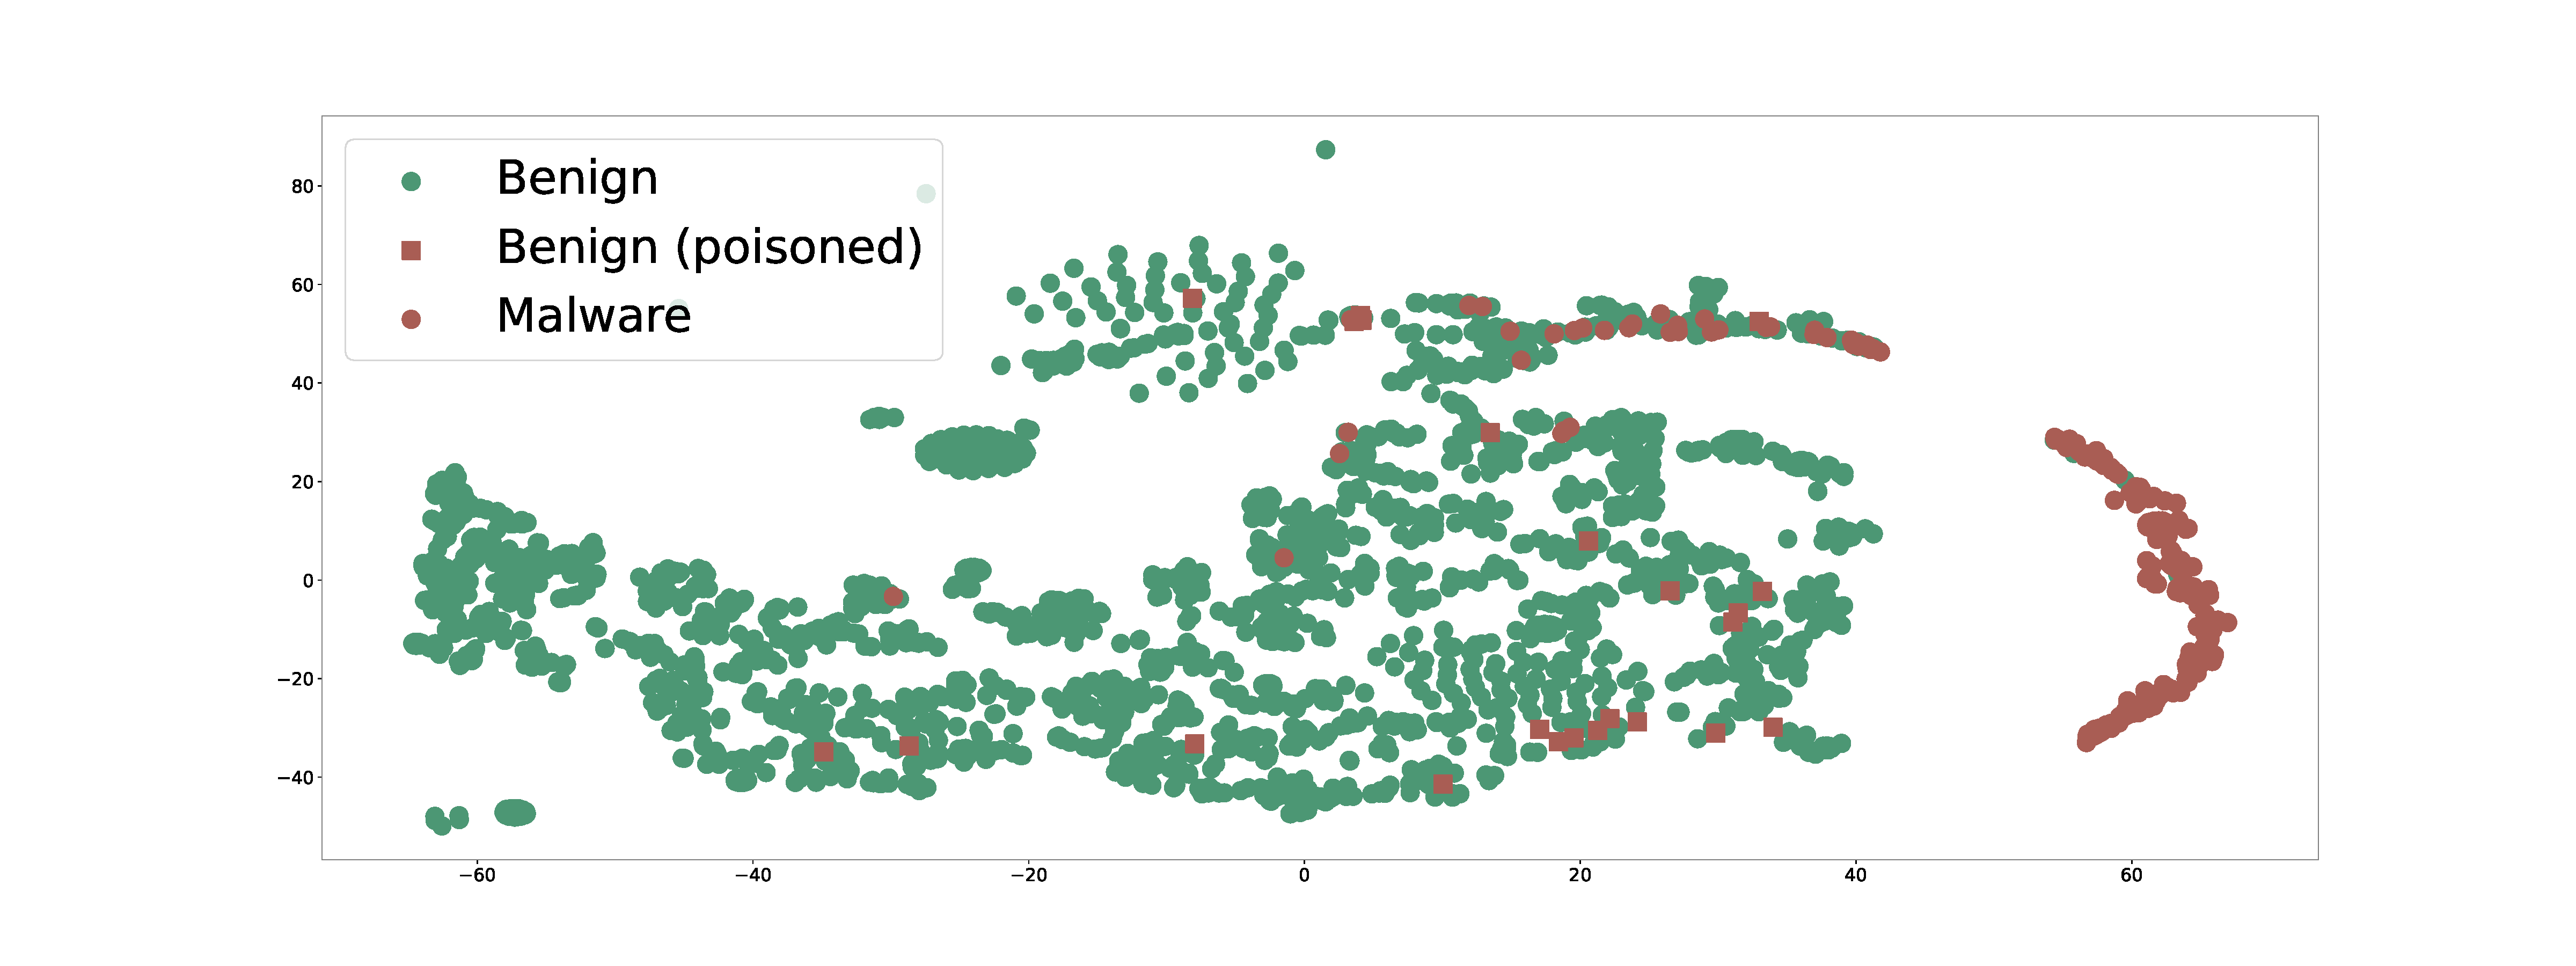
\includegraphics[width=\linewidth,keepaspectratio]{Graph/Evaluation/Figure20.pdf}
	\caption{ICDF Defense Motivation}
	\label{fig:ICDF Defense Motivation}
\end{figure}
Thus, the attack success rate decreases by less than 20\% on average. Specifically, the ASR drops by 16.5\% under the AC defense and 21.8\% under DFP.
Given these limitations, we explore alternative defense strategies in countering \pandora.

Intra-Cluster Distance Filtering (ICDF): In the \pandora, the attacker relies on poisoning seed samples to generate poisoned samples, reducing costs and leading to similarity among the poisoned samples.
Different poisoned samples may originate from the same seed sample.
We measure this similarity using Euclidean distance in the feature space, the basis for our defense method (ICDF).
Unlike AC-based defenses, ICDF filters poisoned samples by exploiting the similarities between the poisoned samples themselves.
%Motivated by this observation, we propose an adaptive sample filtering method based on intra-cluster distance.
%Unsupervised clustering algorithms (e.g., K-means) are applied to the concept drift samples, partitioning the data into $\mathcal{C}$ clusters.
%Each cluster $c \in \mathcal{C}$ contains multiple concept drift samples, and the intra-cluster distance threshold $\tau$ is determined by calculating the mean Euclidean distance between any two samples within the same cluster.
%For each cluster $c$, samples with distances to other samples smaller than the cluster-specific threshold $\tau$ are removed.
So, we propose an adaptive sample filtering method based on intra-cluster distance.
Specifically, using an unsupervised clustering algorithm (e.g., K-means), we partition the concept drift samples into a set of clusters $Clu$ ($Clu= \{c_{1},c_{2},..,c_{k} \}$).
Each cluster $c_{k}$ calculates an intra-cluster distance threshold $\tau$ (Equation~\ref{ICDF Defense Method}) as the mean Euclidean distance $d_{Euc}(\bm{\mathrm{x}}_{i}, \bm{\mathrm{x}}_{j})$ between its samples.
\begin{equation}
	\begin{aligned}
		\tau = \frac{1}{|c_{i}| (|c_{i}| - 1)} \sum_{i \neq j} d_{Euc}(\bm{\mathrm{x}}_{i}, \bm{\mathrm{x}}_{j}) \quad i,j \in c_{k}
	\end{aligned}
	\label{ICDF Defense Method}
\end{equation}
$|c_{i}|$ is the number of samples in the cluster $c_{i}$.
Samples with distances smaller than $\tau$ to others in the same cluster are removed.
%\begin{figure}[t]
%	\centering
%	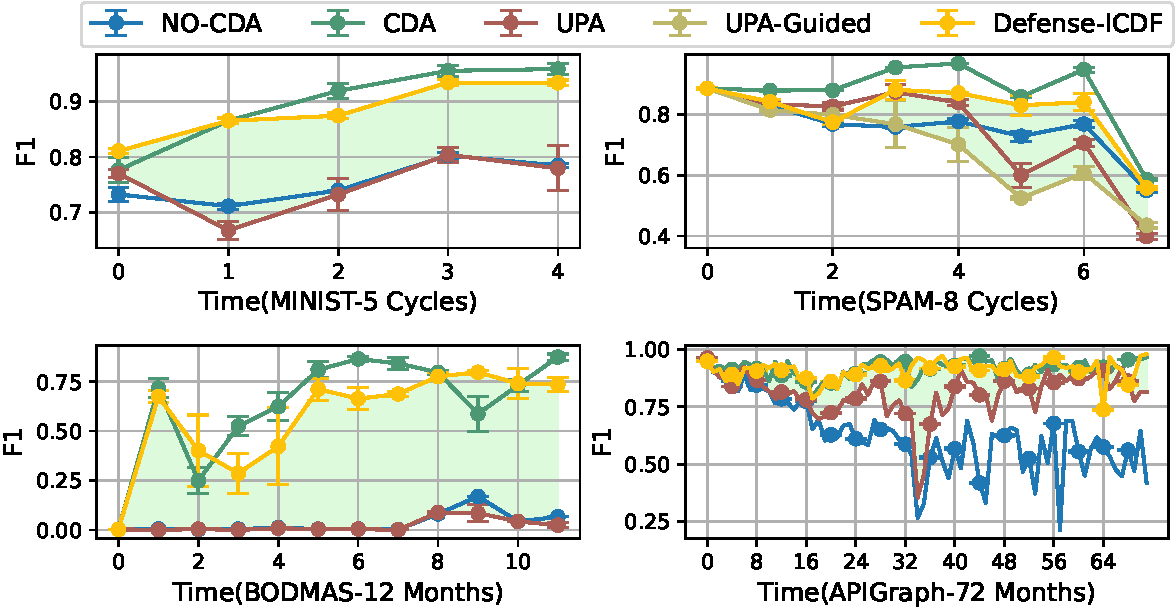
\includegraphics[width=\linewidth,keepaspectratio]{Graph/Evaluation/Figure19_1.pdf}
%	\caption{ICDF Defense (Multi-Target \pandora)}
%	\label{fig:ICDF Defense against Untargeted Poisoning Attack}
%\end{figure}
%\begin{figure}[h!]
%	%\vspace{-0.8em}
%	\centering
%	\subfloat[ICDF Defense Single-Target]{
%		\label{fig11-1}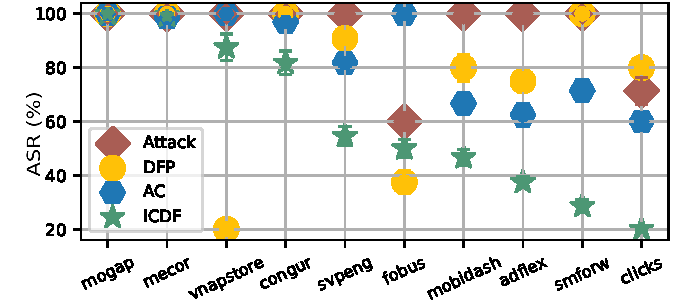
\includegraphics[width=3.90cm, height=2.9cm]{Graph/Evaluation/Figure-last_1.pdf}
%	}
%	\subfloat[ICDF Defense Multi-Target ]{
%		\label{fig11-2}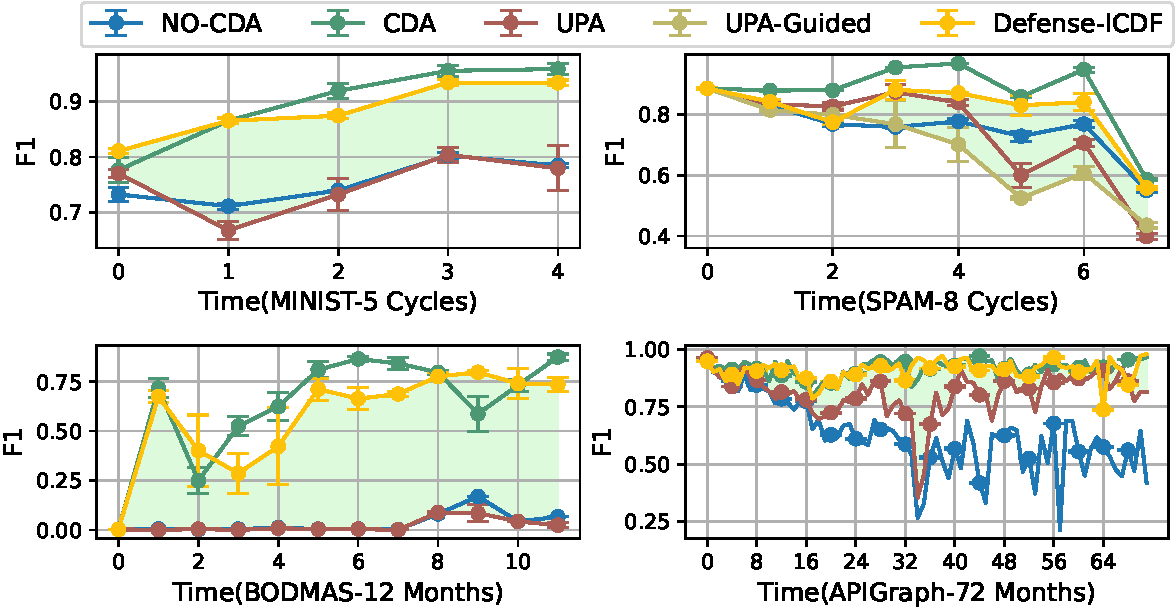
\includegraphics[width=4.60cm, height=2.9cm]{Graph/Evaluation/Figure19_1.pdf}
%	}
%	\caption{xxxxxxxxxxxxx.} 
%	\label{fig111}
%	%\vspace{-1em}
%\end{figure}
%The defense effectiveness against UPA is shown in Figure~\ref{fig:ICDF Defense against Untargeted Poisoning Attack}, demonstrating that the proposed defense method is effective across all four datasets.  
%For clarity, we used green shading to indicate the portion of model performance improvement after applying the ICDF defense method compared to the model performance under attack.
%Notably, in the MNIST and BODMAS datasets, the model performance during certain testing periods even exceeded the optimal performance of concept drift adaptation.  
%This demonstrates that our defense method not only filters out poisoned samples but also enhances the performance of concept drift adaptation itself.
%Among the datasets, the BODMAS dataset exhibited the greatest improvement, with an average F1 increase of 0.52 and a maximum increase of 0.78.
%\textbf{The ICDF defence effectively counters multi-target attack across all four datasets.}
%Green shading highlights performance improvements after applying ICDF, with notable gains in MNIST and BODMAS, where model performance during some periods surpassed the optimal performance of concept drift adaptation.
%The superior performance over the best original concept drift adaptation is due to ICDF's clustering approach, which removes poisoned samples and reduces data redundancy in clean samples, improving training efficiency.
%Although there is a lack of research in the concept drift field, studies in computer vision have shown that data redundancy reduces model training efficiency~\cite{kong2023peeling}.
%Since improving concept drift adaptation is beyond the scope of this study, we will address it in future research.
\begin{figure}[h!]
	\centering
	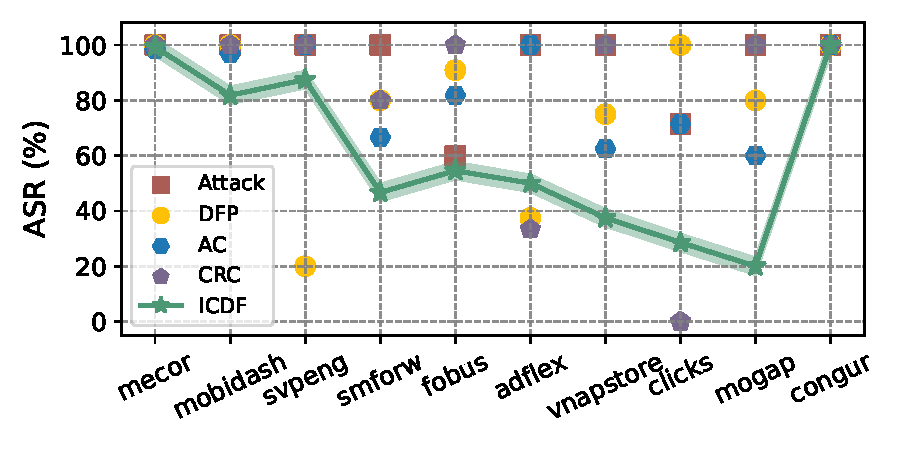
\includegraphics[keepaspectratio,height=3.5cm]{Graph/Evaluation/Figure-last.pdf}
	\caption{ICDF Defense (Single-Target \pandora)}
	\label{fig:APIGraph-targeted-defense}
\end{figure}
ICDF achieved the best defense effect under single-target attack mode, reducing the success rate of \pandora by 39\% across the Top 10 target sets, as shown in Figure~\ref{fig:APIGraph-targeted-defense}. 
While other defense methods demonstrated some effectiveness, they were 20.29\%, 12.43\% and 22.43\% less effective than ICDF, respectively.
We observed that, with the exception of ICDF, which consistently reduced the attack success rate across all attack targets, other defense methods inadvertently increased the attack success rate for certain targets.
%In the fobus family, the other three defense methods resulted in an average increase of 51.72\% in the attack success rate.
Moreover, ICDF effectively reduces the attack success rate of \pandora while causing only a 0.03 drop in F1-score compared to the no-attack scenario, thereby maintaining stable overall concept drift adaptation performance.
We also conducted defensive testing under an enhanced attack strategy that introduces misleading concept drift.
The attack success rate was reduced by 32.6\%, under the same experimental settings as those used in the attack effectiveness evaluation.
We also conducted defense tests against multi-target attacks across four different datasets, as shown in Table~\ref{tab:dma }.
The attack success rate decreased by an average of 54.97\% across the four datasets.
Therefore, our ICDF defense method also demonstrates strong effectiveness in defending against multi-target attack scenarios.
Moreover, after introducing the ICDF defense method, the F1 score on the four datasets was restored to an average of 0.91, indicating that the normal concept drift adaptation performance was not affected.
\begin{table}[htbp]
	\caption{ICDF Defense (Multi-Target \pandora)}
	\label{tab:dma }
	\setlength{\tabcolsep}{5.8pt}
	\begin{center}
		\scalebox{1.0}{
			\begin{tabular}{ccccc}
				\toprule
				\textbf{Datasets}&\textbf{Targets}&\textbf{F1-Attack} &\textbf{F1-Defense} &\textbf{ASR-Decrease} \\
				\midrule
				APIGraph & 734  &  0.76 & 0.90\textsubscript{\textcolor{red}{\textbf{+0.14}}} & 21.26\% \\ 
				\specialrule{0.05em}{1pt}{1pt}
				MNIST & 1,398  & 0.78 & 0.82 \textsubscript{\textcolor{red}{\textbf{+0.04}}}& 75.47\%\\
				\specialrule{0.05em}{1pt}{1pt}
				BODMAS & 222  &  0.92 & 0.99\textsubscript{\textcolor{red}{\textbf{+0.07}}} &54.05\% \\ 
				\specialrule{0.05em}{1pt}{1pt}
				SPAM & 168  &  0.91 & 0.94\textsubscript{\textcolor{red}{\textbf{+0.03}}} &69.04\% \\ 
				\bottomrule
		\end{tabular}}
	\end{center}
\end{table}

To better demonstrate the effectiveness of the ICDF method, we analyze the variation in defense performance under different parameter settings.
We selected the APIGraph dataset, which spans the longest time period, for defense parameter analysis.
The number of clusters was the only parameter requiring manual configuration during the defense.
We conducted analyses under both single-target and multi-target attack scenarios.  
We evaluated four cluster settings (6, 10, 20, and 40) under the multi-target attack. 
The mean F1 score across these four settings was 0.91, with a variance of 0.0025.
Given the large number of attack targets in the single-target setting, we selected a subset of representative malware families for detailed evaluation.
In the single-target attack, we selected the family 'clicks' (with the best ICDF defense performance) and the family 'mogap' (with the worst ICDF defense performance) from the Top 10 attack targets.
For each family, we conducted four experiments with clustering parameter settings of 6, 10, 20, and 40 and observed that the defense performance remained consistent across all settings.
This indicates that the defense parameter settings have minimal impact on defense effectiveness, which can effectively reduce the deployment costs of the defense method.